Systém \gls{mtb} vznikl okolo roku 2000, kdy se hledal vhodný systém pro
programovatelné počítačové řízení modelové železnice, spoluprací nadšenců
z~\textit{Klubu modelářů železnic Brno I} (dále jen \gls{kmz}) a \textit{Klubu
železničních modelářů Praha 3} \footnote{Je překvapivé, že
skupina nadšenců tehdy dokázala vytvořit systém, který by se mohl poměřovat se
současnými komerčními systémy řízení modelových kolejišť, viz dále.} \cite{mtb:web}.

\textit{Digital Command Control} (\gls{dcc}), dnes pravděpodobně
nejrozšířenější\footnotemark\\mezinárodně standardizovaný systém pro digitální
řízení modelové železnice \cite{dcc_intro:web}, tehdy ještě nebyl v~České republice
rozšířený. Navíc přirozeně vyvstal požadavek na minimalizaci nákladů
a maximalizaci nezávislosti na komerčních produktech rodiny jednoho výrobce. Vznikl
tedy systém \gls{mtb}, který se pro řízení modelových kolejišť v \gls{kmz}
používá doposud \cite{kmz_rizeni:web}. Podotkněme, že systém \gls{mtb} se
do~dalších klubů po České Republice nerozšířil – nejspíš proto, že není
podporovaný komerčními softwary pro řízení modelové železnice a~že jej jeho
původní autor v~roce~2008 přestal udržovat.

\footnotetext{Autor této práce by rád odstranil slovo
\textit{pravděpodobně} a uvedl řádnou citaci. Bohužel neexistují studie, které
by bylo možné citovat. Rozšířenost \gls{dcc} se zakládá na autorových
zkušenostech.}

\section{Popis systému MTB} \label{sec:mtbbus}

Systém \gls{mtb} se skládá z:

\begin{compactenum}
\item sběrnice \gls{mtbbus},
\item \textit{\gls{mtb} modulů},
\item \textit{\gls{mtbusb}} modulu,
\item počítačových knihoven pro přístup k~\gls{mtbusb}.
\end{compactenum}

Každé kolejiště má svou vlastní sběrnici \gls{mtbbus}, ke které je připojený
právě jeden \gls{mtbusb} modul a až 255 \gls{mtb} modulů.
\gls{mtbusb} řídí provoz sběrnice \gls{mtbbus} a~je připojen k~počítači.
\gls{mtb} moduly jsou pevně instalovány v~rámech kolejiště a~komunikují po
sběrnici \gls{mtbbus} s~\gls{mtbusb} modulem. Říkáme, že sběrnice je tzv.
\textit{single master, multiple slaves}. \gls{mtbusb} modul lze označit jako
\textit{master modul}, \gls{mtb} moduly jsou tzv. \textit{slave moduly}.
Celou situaci přehledně ilustruje obrázek \ref{fig:mtbbus-topology}.

\begin{figure}[ht]
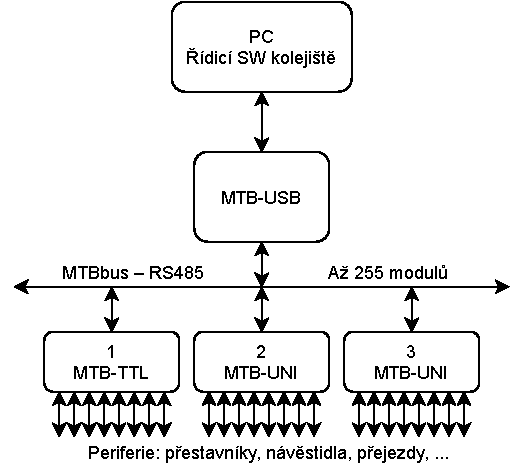
\includegraphics[width=0.7\textwidth]{data/mtb-topology.pdf}
\caption{Topologie systému \gls{mtb}.}
\label{fig:mtbbus-topology}
\end{figure}

Současná sběrnice \gls{mtbbus} je založena na elektrickém standardu
\textit{RS485} \cite{mtbbus-specs}. Sběrnice RS485 je dvouvodičová (\textit{R+,
R-, GND}) vícebodová sériová poloduplexní komunikační průmyslová sběrnice
vyvinutá s~důrazem na odolnost vůči externímu rušení. Je vhodná pro přenos dat
na větší vzdálenosti, řádově až stovky metrů \cite{rs485-specs}. Pro dosažení
nejlepších elektrických vlastností by sběrnice měla být lineární. Sběrnice je
na obou koncích terminována rezistorem \textit{200 R} a~pull-up a~pull-down
rezistory pro držení definované úrovně signálu.

\begin{table}[h]
	\begin{tabularx}{\textwidth}{XX}
		\toprule
		Typ přenosu & RS485, formát dat UART \\
		Komunikační rychlost & 38400~Bd, 57600~Bd, 115200~Bd \\
		Maximální počet modulů & 255 \\
		Počet datových bitů & 9 \\
		Stop bit & 1 \\
		Parita & žádná \\
		Maximální délka vedení & 100 m \\
		\bottomrule
	\end{tabularx}
	\caption{Základní parametry sběrnice \gls{mtbbus} \cite{mtbbus-specs}}
	\label{tab:mtbbus-params}
\end{table}

RS485 je velice snadno implementovatelná do prakticky všech mikrokontrolérů –
pro přístup ke sběrnici je třeba rozhraní UART, jeden pin pro řízení směru
komunikace a driver k~RS485.

Po sběrnici se komunikuje pevně definovaným protokolem. Protokol definuje
příkazy pro moduly, odpovědi modulů, časování apod. \cite{mtbbus-specs}

Základní parametry \gls{mtbbus} shrnuje tabulka \ref{tab:mtbbus-params}.

Zaměřme se nyní na \gls{mtb} moduly. Každý \gls{mtb} modul má:

\begin{compactenum}
\item 8bitovou adresu, která se konfiguruje \textit{jumpery} přímo na modulu,
\item konfiguraci (typ vstupů/výstupů, rychlost sběrnice, ...),
\item vstupy (stav vstupů),
\item výstupy (stav výstupů).
\end{compactenum}

\gls{mtb} moduly mohou být různého typu:

\begin{itemize}
\item \textbf{\gls{mtbuni}}

	\gls{mtbuni} (\textit{univerzální}) je nejpoužívanější typ modulu. Obsahuje
	16~digitálních vstupů a~16~digitálních výstupů. Na výstupech 0–7 umožňuje
	kódovat návěst protokolem \gls{scom}\footnote{\gls{scom} je jednoduchý jednosměrný
	komunikační protokol, který umožňuje přenášet návěsti návěstidel
	\cite{scom-specs}.}, což umožňuje připojení až 8 návěstidel k~jednomu
	\gls{mtbuni}. Modul dále umožňuje připojení \gls{ir} čidel na
	vstupy\footnote{\gls{ir} čidla jsou bodová čidla detekující průjezd vlaku, viz
	\ref{sec:ir}.}. Výstupy modulu jsou v~režimu otevřeného kolektoru
	s~maximální zátěží až 0.5~A~/~8~výstupů.\footnote{Na modulu jsou osazeny
	2~budiče výstupů, přičemž každý z~budičů má celkový limit $0.5$~A.}

\item \textbf{MTB-UNIm}

	MTB-UNIm modul je zjednodušením \gls{mtbuni} modulu. Nemá podporu \gls{ir}
	čidel, ale má výstupy v~režimu otevřených kolektorů. Umožňuje připojení až
	8 S-COM návěstidel.

\item \textbf{MTB-TTL}

	\begin{figure}[ht]
	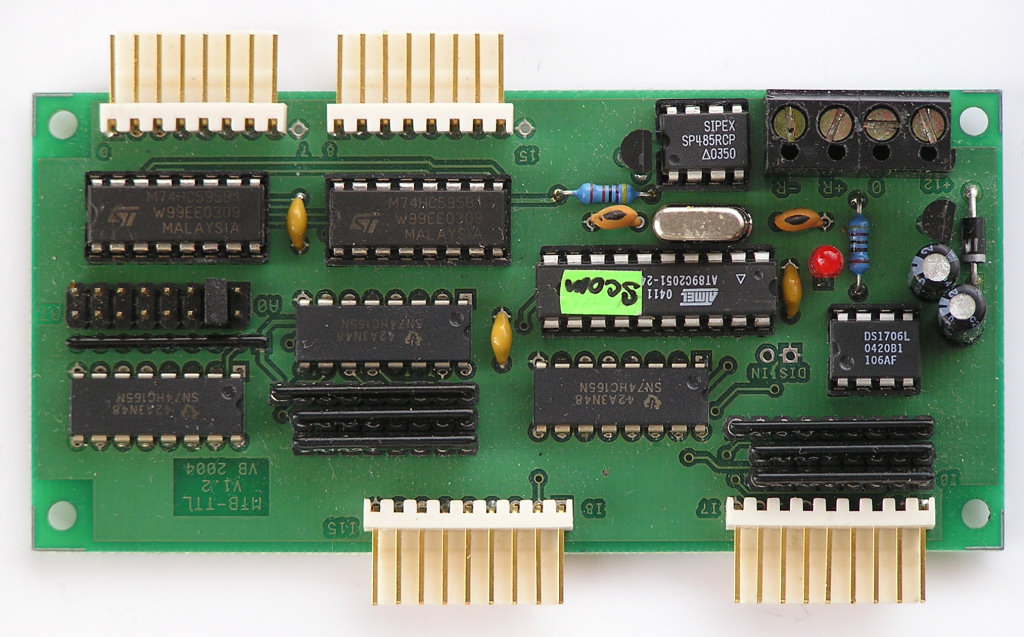
\includegraphics[width=0.7\textwidth]{data/mtbttl_foto.jpg}
	\caption{Ukázka modulu MTB-TTL \cite{mtb:web}.}
	\label{fig:mtbttl}
	\end{figure}

	MTB-TTL je zjednodušením modulu \gls{mtbuni}. Oproti \gls{mtbuni}
	nemá podporu \gls{ir} čidel a~výstupy má v~režimu \gls{ttl}. Od tohoto typu
	modulu se v~současnosti ustupuje, neboť \gls{ttl} výstupy nejsou vhodné pro
	spínání vyšších napětí\footnote{Např. pokud periferie na výstupu obsahuje
	pull-up do +12~V.}, a~proto, že v~případě neaktivního výstupu (neaktivní =
	+5~V; inverzní logika) aktivně napájí výstupní port, což způsobuje nechtěné
	chování, například pokud je na výstupním portu záměrně vypnutá periferie.
	V~krajním případě může dojít až k~přetížení TTL výstupu a jeho zničení. Na
	výstupy všech nasazených moduly typu MTB-TTL byly postupně instalovány
	dodatečné budiče s~otevřenými kolektory.

\item \textbf{MTB-REG}

	MTB-REG je modul umožňující generovat analogový výkonový výstup. Modul se
	připojí ke kolejím a řídí rychlost a~směr lokomotivy v~řízeném úseku kolejí.

	Tento způsob řízení jízdy (tzv. \textit{analogový}) je dnes již překonaný.
	V~současnosti se pro řízení jízdy lokomotiv na kolejišti používá tzv. systém
	\textit{Digital Command Control} (viz \ref{sec:dcc}), kde každá lokomotiva
	a mnohdy i~vagón v~sobě má mikroprocesor a~celý systém je řízen
	digitálně \cite{dcc_intro:web}.

	Modul MTB-REG je tedy již překonaným modulem a~autor jej uvádí především pro
	úplnost popisu systému \gls{mtb}.

\item \textbf{MTB-POT}

	Modul MTB-POT obsahuje 4 analogové vstupy a 4 digitální vstupy. Jeho
	původním účelem bylo, aby se připojil k~potenciometru v~pultu obsluhy
	kolejiště, kterým obsluha reguluje jízdu vlaku. Po sběrnici přepošle data
	modulu MTB-REG a~tím dojde ke kýžené jízdě vlaku. Tento způsob řízení jízdy
	na kolejištích se již nepoužívá, proto i~modul MTB-POT na moderních
	kolejištích pozbývá svého smyslu.

\end{itemize}

Práce se sběrnicí z~pohledu aplikace v~počítači probíhá následovně:

\begin{compactenum}
\item Aplikace se připojí k~\gls{mtbusb} modulu.
\item Aplikace provede sken aktivních modulů sběrnice.
\item Aplikace nahraje do všech aktivních modulů konfiguraci.
\item Aplikace přečte stav vstupů.
\item Aplikace zahájí provoz sběrnice – od této chvíle všechny moduly nahlašují
	změny stavů vstupů.
\item Aplikace čte vstupy, nastavuje výstupy a řídí provoz.
\item Aplikace ukončí provoz sběrnice a vynuluje stav výstupů \gls{mtb} modulů.
\item Aplikace uzavře spojení s~\gls{mtbusb}.
\end{compactenum}


\section{IR čidla} \label{sec:ir}

Nyní popíšeme princip fungování \gls{ir} čidel v~kolejišti, protože bude v~dalších
kapitolách stěžejní.

\gls{ir} čidlo je bodový detektor průjezdu vlaku. Do kolejí se vedle sebe umístí
opticky oddělená vysílací dioda a~fototranzistor, oba namířené vzhůru. Při
průjezdu vlaku dojde k~odrazu signálu od spodní části vozu nebo lokomotivy,
čímž je detekován průjezd vlaku. Výhodou je nenápadná instalace mezi kolejové
pražce, která neruší celkový dojem modelu.

Pro spolehlivou detekci odrazu od matných černých povrchů podvozků je třeba
budit vysílací diodu vysokým proudem (až 200~mA), což vyžaduje použití
diody v~impulsním režimu. Současná \gls{mtbuni} deska podporuje \gls{ir} čidla na
všech svých 16 vstupech, diody jsou buzeny tranzistory ve skupinách po
4~diodách.

Aby bylo zajištěno spolehlivé vyhodnocení odraženého signálu, je vstup
z~fototranzistoru zapojen na digitální vstup posuvného registru přes kapacitní
vazbu (viz schéma \ref{fig:cap-bind}). Kapacitní vazba odstraňuje stejnosměrnou
složku signálu, která vzniká vlivem okolního osvětlení.

\begin{figure}[ht]
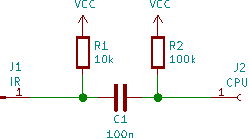
\includegraphics[width=0.5\textwidth]{data/cap-bind/capacitive-bind-example.pdf}
\caption{Zapojení vstupu kapacitní vazbou.}
\label{fig:cap-bind}
\end{figure}

Vstupy \gls{mtbuni} desky se konfigurují osazením rezistorů (běžný
vstup) nebo kondenzátorů (vstup z~\gls{ir} čidla). Režim pinu musí být
uložený v~procesoru, aby se adekvátním způsobem zpracovával vstupní signál
\cite{mtbuni22-specs}.


\section{Systém \gls{mtb} v~kontextu řízení modelového kolejiště} \label{sec:mtb_context}

V~\gls{kmz} je aktuálně systém \gls{mtb} nasazen na dvou kolejištích, další
nasazení je na modulovém kolejišti Mendelovy univerzity v~Brně, s~kterou klub
spolupracuje. Na těchto kolejištích je aktuálně nasazeno 99 \gls{mtb} desek.

Pro kontext uveďme, jak systém \gls{mtb} zapadá do celkové koncepce řízení
kolejiště. Viz schéma \ref{fig:control-topology}.

\begin{figure}[ht]
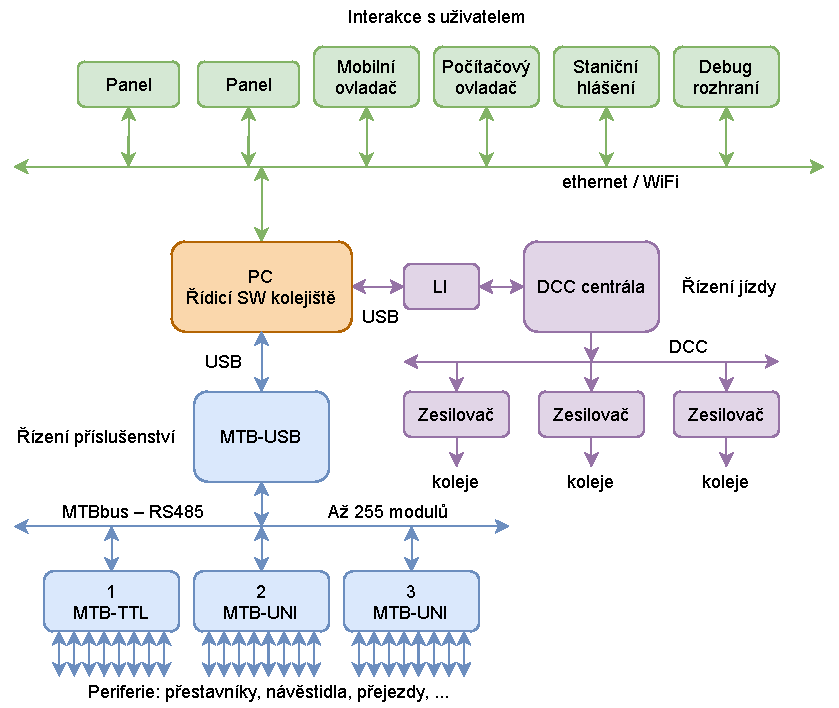
\includegraphics[width=\textwidth]{data/railroad-diagram.pdf}
\caption{Schéma komponent řízení kolejiště v~\gls{kmz}.}
\label{fig:control-topology}
\end{figure}

Na první pohled je vidět, že kolejiště je řízeno dvěma různými systémy:
systémem pro řízení příslušenství (modrá část diagramu) a~systémem pro řízení
jízdy (fialová část diagramu). Vyvstává otázka, proč je nesloučit do systému
jednoho. Integrovaná řešení nabízejí majoritní výrobci hardwaru pro digitální
řízení modelové železnice. Řízení jízdy i~příslušenství jedním systémem (\gls{dcc})
je rozšířeným řešením jak v~Česku tak v~zahraničí. Všechna tato řešení jsou
však o~kompromisech, jak se dozvíme v~\ref{sec:dcc}.

U~tvorby a~nasazení systému \gls{mtb} stály osoby, které pracují na zabezpečení
skutečné železnice. Systém \gls{mtb} je tak oproti komerčně dostupným řešením
řízení modelových kolejišť navrhován s~důrazem na spolehlivost a~především
bezpečnost.

Uveďme dva příklady za všechny: komerčně využívaná sběrnice RS pro snímání
stavu kolejiště nedokáže rozpoznat, že nějaký z~RS modulů (analogie \gls{mtb}
modulů) přestal pracovat \cite{rs:web}. Dále výstupní moduly nijak nepotvrzují,
že opravdu provedly akci, kterou počítač požaduje \cite{dcc_specs:web}. Tyto
příklady ilustrují, že komerčně dostupná řešení jsou podle autorova názoru blíže
hračce, než bezpečnému a~spolehlivému systému pro řízení modelů.

Poslední část schématu \ref{fig:control-topology} je část zelená, která
reprezentuje interakci s~uživatelem. \textit{Řídicí SW kolejiště} běží na
samostatném serveru, ke kterému se připojují všichni uživatelé systému –
dispečeři ze svých stanic, strojvedoucí ze svých ovladačů, ale také třeba
technikové se svými diagnostickými nástroji nebo externí programy využívající
\gls{api} serveru. Server kontroluje identitu uživatelů a umožňuje jim řídit ty
systémy, ke kterým mají uživatelé práva.

\section{Proč současný systém \gls{mtb} nedostačuje} \label{sec:mtb_fail}

Systém \gls{mtb} s~sebou nese řadu problémů.

\begin{enumerate}
\item \textbf{Licence, výrobní data}

U~současné implementace systému \gls{mtb} bohužel nebyly řádně vyřešeny licenční
podmínky mezi jeho autorem a~Klubem. Souhrou událostí se \gls{kmz} dostal do
situace, kdy nemá zdrojová data schémat a~layoutů desek plošných spojů ani
zdrojové kódy firmwarů.

Aktuální situace tak prakticky znemožňuje výrobu dalších \gls{mtb} desek,
o~záměru chtít systém \gls{mtb} nabízet mimo klub ani nemůže být řeč.

\item \textbf{Hardware}

Systém \gls{mtb} zaznamenal poslední aktualizaci hardwarových komponent v~roce
2007. V~současné době jsou některé použité součástky bohužel nedostupné, což
znemožňuje výstavbu dalších částí kolejiště. To je zcela zásadní problém.

\item \textbf{Software}

Současné MTB moduly využívají procesory \textit{AT89C2051} (2~kB FLASH,
128~B SRAM). Tyto procesory svými parametry odpovídají době návrhu celého
systému. Firmware v~procesorech naráží na jejich hardwarové limity – paměť
je plná, takže nelze přidávat nové funkce. Procesorům navíc chybí některé
klíčové periferie, například EEPROM paměť.

\end{enumerate}

Současný systém \gls{mtb} byl vyhodnocen jako celkově nedostatečný, je potřeba
ho buď aktualizovat nebo nahradit za systém jiný.

\subsection{Všeobecné požadavky na nový systém \gls{mtb}} \label{subsec:gen_requirements}

Na náhradu systému \gls{mtb} autor práce stanovil především následující
požadavky.

\begin{compactenum}
\item Systém musí být kompatibilní se současným řídicím softwarem kolejiště.
\item Systém musí být kompatibilní se současným hardwarem kolejiště.
\item Systém musí být udržitelný minimálně 20~let.
\item Finanční náklady a~čas vložený do povýšení současného systému na nový
	systém by měly být minimalizovány.
\item Systém musí být schopen potvrzovat akce řídicího počítače a~evidovat správnou
	funkčnost modulů.
\item Systém by měl být rozšiřitelný co se týče podporované funkcionality –
	nové požadavky by mělo být možné implementovat.
\end{compactenum}

K~naplnění těchto požadavků lze přistoupit dvěma různými způsoby: zakoupením
komerčního produktu nebo vytvořením produktu vlastního. Prozkoumejme nejprve,
jestli existují komerční řešení, která naplňují definované požadavky.
